% =====================================================================================
% sections/ext_defence.tex: material cut from sections/defence.tex (extended version only).
% Appendix-ready: \subsection headings only; place it after appendix_defence.tex.
% Where each block came from (the draft of sections/defence.tex of 2026-10-10, before the cut):
%   "The Integer Model: Execution Details"  <- Sec. 4.1, paragraphs "Weight operations",
%       "Operations without weights" and "Exact execution" (im2col and BatchNorm folding, the
%       requantisation formula, the last-position LM head, int8 inputs, hardware errors).
%   "Commitment Plans"  <- Sec. 4.2, paragraph "Commitment plans" and the domain separation of
%       the Merkle trees (six candidate plans, LeNet-5 example, stacking of q/k/v projections).
%   "The Fiat--Shamir Transcript"  <- Sec. 4.4, paragraph "A sponge transcript" (32-byte keys,
%       rejection sampling) and the requantisation-multiplier example.
%   "Untrusted Commitments: Measurements, Trade-off and Scope"  <- Sec. 4.5, paragraphs "The
%       split-commitment attack" (300-query measurement), "A one-time setup proof" (transposed
%       matrices), "The trade-off" with Table tab:setup, and "Scope".
% Labels defined: tab:setup (moved here from defence.tex). Labels used: sec:intmodel, sec:fs,
%   eq:split, thm:untrusted (defence.tex); app:semantics, app:sound, app:untrusted
%   (appendix_defence.tex). New BibTeX key: fri2018 (also cited in defence.tex).
% =====================================================================================

\providecommand{\F}{\mathbb{F}_p}
\providecommand{\sC}{\mathsf{C}}
\providecommand{\para}[1]{\par\noindent\textbf{#1}\quad}
\providecommand{\todo}[1]{\textbf{[TODO: #1]}}
\providecommand{\toprule}{\hline}
\providecommand{\midrule}{\hline}
\providecommand{\bottomrule}{\hline}

\subsection{The Integer Model: Execution Details}

Floating-point results depend on the device and on the order of summation, and a tolerance would
leave a cheating prover room to hide small changes. The defence therefore certifies the integer
model of Section~\ref{sec:intmodel}. Its weight operations come from the layers of the network as
follows. Convolutions become products through im2col, with one column of $X_\ell$ per pixel.
BatchNorm is folded into $W_\ell$ and $b_\ell$, and the scales of the weights are absorbed into the
integer multiplier of the next requantisation. A requantisation with multiplier $m$ computes
$\mathrm{clamp}(\lfloor(mz+2^{29})/2^{30}\rfloor,-127,127)$; Appendix~\ref{app:semantics} gives
every other operation without weights.

For a language model the output $y$ is the vector of next-token logits. These depend only on the
last position, so the last block is computed there alone, except for the keys and values that
attention reads.

Every weight operation's input is int8, since it comes from a clamped requantisation, a table or a
norm. The prover therefore runs $W_\ell X_\ell$ on int8 tensor cores: products are at most
$2^{14}$ in magnitude, and blocks of $2^{16}$ of them sum exactly in 32-bit integers. Attention
runs in float32 within its exact range (Appendix~\ref{app:semantics}). A hardware error can only
make an honest proof fail.

\subsection{Commitment Plans}

Each Merkle tree hashes its leaves and its inner nodes with separate domain prefixes. $C_M$ uses
no secret randomness, so anyone who holds the weights can recompute it. Long codewords need fewer
opened columns, and matrices whose codewords have equal length can share one tree and one Merkle
multiproof. The public planning rule chooses among six candidate plans of codeword lengths and
layouts. The five weight matrices of LeNet-5, for example, share one tree of $2^{18}$ positions and
open 15 columns, instead of 66 in each of five trees. In the transposed layout, operations that
read the same input, such as the query, key and value projections, are stacked into one matrix.

\subsection{The Fiat--Shamir Transcript}

Interactively, each challenge is expanded with SHAKE-256 from a fresh 256-bit key that the
verifier draws. Under Fiat--Shamir the keys are derived from the transcript instead. The
transcript is a SHAKE-256 sponge with a protocol-specific domain string, and messages are absorbed
with labels and length prefixes, so its encoding is injective. A challenge key is 32 bytes
squeezed from a copy of the sponge after it absorbs the challenge's label. Rejection sampling
expands it into unbiased field elements and distinct column indices. Two models that differ in one
requantisation multiplier have different graph digests and thus produce different challenges. A
prover that rehashes altered claims in search of favourable challenges is covered by the factor
$Q$ of the Fiat--Shamir bound of Section~\ref{sec:fs}; the round-by-round states are defined in
Appendix~\ref{app:sound}.

\subsection{Untrusted Commitments: Measurements, Trade-off and Scope}

\para{The split commitment in practice.} For the smallest tree of Llama-2-7B ($t=35$),
Eq.~\eqref{eq:split} gives an acceptance probability of about $2^{-35}$ per query, not $2^{-128}$.
On a small decoder with one weight row changed in one operation, the acceptance rate over 300
queries with a small $t$ matched Eq.~\eqref{eq:split}. Against a malformed commitment a column is
worth about one bit instead of $\log_2(n_j/k_j)$, so per-query checks alone would need
3.2--6.6$\times$ the column bytes on the models of Table~\ref{tab:setup}. Our implementation
rejects the setup proof of the split commitment, which is not $e_j$-close for
$e_j<n_j/2-k_j+1$ (Appendix~\ref{app:untrusted}).

\para{Transposed matrices.} The per-query combination $[X;\mathbf 1]\chi'$ of a transposed matrix
lies in the span of the activations and is not uniform, so it cannot establish closeness. The
setup proof is therefore required for transposed matrices.

\para{The trade-off.} A larger radius $e_j$ shortens the setup proof, since each setup column then
catches a far matrix with probability about $e_j/n_j$, and lengthens every query, whose bound in
Theorem~\ref{thm:untrusted} has $k_j+e_j$ in place of $k_j$. Each tree takes the radius, among the
fractions $2^0,\dots,2^{-10}$ of the unique-decoding radius, that minimises $t^0_j/a+t_j$ over $a$
amortised queries (Table~\ref{tab:setup}; the parameters are derived in
Appendix~\ref{app:untrusted}). At $a=1{,}000$, Llama-2-7B pays 11.3\,GB once and 8\% more column
bytes per query; at 2{,}048 tokens the change per query is below 1\%. Our implementation covers
commitment plans, including shared trees and transposed matrices. \todo{L40S: setup prover and
verifier time for GPT-2 and the 7B models}

\begin{table}[t]
  \caption{Untrusted commitments at $\lambda=128$: the one-time setup proof and the opened columns
  per query, with setup parameters amortised over $a=100$ or $1{,}000$ queries (interactive
  queries, 4 bytes per field element)}
  \label{tab:setup}
  \centering
  \footnotesize
  \setlength{\tabcolsep}{3.5pt}
  \begin{tabular}{lrrrr}
    \toprule
    & \multicolumn{2}{c}{setup proof} & \multicolumn{2}{c}{columns per query (MB)} \\
    Model & $a{=}100$ & $a{=}1{,}000$ & honest & untrusted, $a{=}100$ / $1{,}000$ \\
    \midrule
    GPT-2       & 213\,MB & 686\,MB  & 3.22  & 6.84 / 4.63 \\
    Llama-2-7B  & 2.8\,GB & 11.3\,GB & 124.7 & 168.5 / 134.9 \\
    OPT-6.7B    & 2.5\,GB & 10.2\,GB & 85.9  & 130.7 / 97.1 \\
    Llama-2-13B & 4.0\,GB & 16.4\,GB & 149.3 & 217.4 / 165.9 \\
    \bottomrule
  \end{tabular}
\end{table}

\para{Scope.} Neither the setup proof nor mode $\sC$ hides the weights: the verifier knows $X_\ell$
and $Z_\ell$, so the claims of about $\lceil k_\ell/T\rceil$ queries reveal $A_\ell$. Mode $\sC$
thus suits weights that the client may see. When the int8 model can be recomputed from the public
checkpoint and recipe, recomputing $C_M$ also settles which model is committed, and it is cheaper
than a setup proof, which for GPT-2 is larger than the int8 weights. The setup proof serves
clients that cannot have $C_M$ recomputed. It opens whole columns; a batched proximity proof over
the rows in the style of FRI~\cite{fri2018} or BaseFold~\cite{basefold} could replace them, but we
have not evaluated one.

% Moved from defence.tex (Sec. 4.3) for space.
\subsection{One Query in Mode $\sC$}
Figure~\ref{fig:protocol} shows the three rounds of one query in mode $\sC$ with an honest commitment.
\begin{figure}[t]
  \centering
  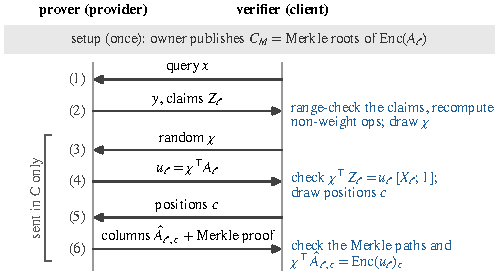
\includegraphics[width=\columnwidth]{figures/protocol.pdf}
  \caption{One query in mode $\sC$ with an honest commitment. Each value is fixed before the
  randomness that tests it}
  \label{fig:protocol}
\end{figure}
